%---------------------------------------------------------------------
%
%                          Anexo A
%
%---------------------------------------------------------------------

\chapter{Tabla de puntuaciones individuales y examen de prueba}
\label{anexoA}

\begin{resumen}
	En este anexo se recoge la tabla de puntuaciones individuales para cada requisito de cada miembro del equipo de desarrollo, as� como el examen de prueba proporcionado en la evaluaci�n de la aplicaci�n.
\end{resumen}

\begin{longtable}[c]{|p{7.3cm}|c|c|c|}
	\hline
	\multicolumn{1}{|c|}{\multirow{2}{*}{\textbf{Requisito}}} & \multicolumn{3}{c|}{\textbf{Puntuaci�n}} \\ \cline{2-4} 
	\multicolumn{1}{|c|}{} & \textbf{Jorge} & \textbf{Natalia} & \textbf{Pablo} \\ \hline
	\endfirsthead
	%
	\multicolumn{4}{c}%
	{{\bfseries Tabla \thetable\ continuada de la p�gina anterior}} \\
	\endhead
	%
	Generar un resumen a partir de un texto & 3 & 2 & 2 \\ \hline
	Crear esquemas que faciliten la visualizaci�n del temario y/o las actividades, seleccionando contenido de un texto ya redactado o escribiendo desde cero & \multirow{4}{*}{2} & \multirow{4}{*}{1} & \multirow{4}{*}{2} \\ \hline
	Crear tablas que organicen el temario y/o las actividades, seleccionando contenido de un texto ya redactado o escribi�ndolo desde cero & \multirow{4}{*}{2} & \multirow{4}{*}{1} & \multirow{4}{*}{2} \\ \hline
	Ejercicios de relacionar contenido mediante flechas & \multirow{2}{*}{2} & \multirow{2}{*}{2} & \multirow{2}{*}{2} \\ \hline
	Ejercicios de sopa de letras & 3 & 3 & 3 \\ \hline
	Ejercicios de completar espacios en un texto & 2 & 2 & 3 \\ \hline
	Ejercicios de pregunta de desarrollo con un espacio limitado para escribir la respuesta & \multirow{2}{*}{2} & \multirow{2}{*}{2} & \multirow{2}{*}{3} \\ \hline
	Ejercicios de verdadero o falso & 3 & 3 & 3 \\ \hline
	Ejercicios de completar los espacios en blanco en tablas & \multirow{2}{*}{2} & \multirow{2}{*}{2} & \multirow{2}{*}{2} \\ \hline
	Ejercicios de completar los espacios en blanco en esquemas & \multirow{2}{*}{1} & \multirow{2}{*}{1} & \multirow{2}{*}{1} \\ \hline
	A�adir enunciados y ejemplos (con o sin pictogramas), donde se explique c�mo debe resolverse el ejercicio & \multirow{3}{*}{3} & \multirow{3}{*}{3} & \multirow{3}{*}{3} \\ \hline
	Sustituir una palabra por un pictograma & 3 & 2 & 3 \\ \hline
	Sustituir una palabra por una imagen & 2 & 2 & 3 \\ \hline
	Resaltar una palabra con un color & 3 & 3 & 3 \\ \hline
	A�adir una  leyenda de colores con la categor�a de cada tipo de palabra resaltada, para que los alumnos puedan identificar el significado de cada una de las palabras resaltadas en el texto & \multirow{4}{*}{3} & \multirow{4}{*}{3} & \multirow{4}{*}{3} \\ \hline
	A�adir una leyenda de colores para el tema de cada asignatura, para que los alumnos las distingan con mayor facilidad & \multirow{3}{*}{3} & \multirow{3}{*}{3} & \multirow{3}{*}{3} \\ \hline
	Estandarizar formato en textos, estableciendo una fuente de texto determinada y un tama�o acorde para cada alumno & \multirow{3}{*}{3} & \multirow{3}{*}{1} & \multirow{3}{*}{2} \\ \hline
	Estandarizar formato para t�tulos e �ndices del temario, generando de forma autom�tica una plantilla del color de la asignatura & \multirow{3}{*}{3} & \multirow{3}{*}{1} & \multirow{3}{*}{2} \\ \hline
	Aumentar el tama�o de la fuente de una parte del texto & \multirow{2}{*}{3} & \multirow{2}{*}{2} & \multirow{2}{*}{3} \\ \hline
	Subrayar una parte del texto & 3 & 2 & 3 \\ \hline
	Poner en negrita una parte del texto & 3 & 2 & 3 \\ \hline
	A�adir im�genes buscando una palabra en bases de datos de im�genes libres & \multirow{2}{*}{2} & \multirow{2}{*}{3} & \multirow{2}{*}{2} \\ \hline
	A�adir espacio extra entre l�neas para escribir & \multirow{2}{*}{2} & \multirow{2}{*}{2} & \multirow{2}{*}{2} \\ \hline
	\caption{Puntuaci�n individual de cada miembro del equipo de desarrollo para cada requisito}
	\label{tabla:anexoA:puntuacionIndividual}\\
\end{longtable}

%\begin{figure}[h!]
%	\centering
%	
%		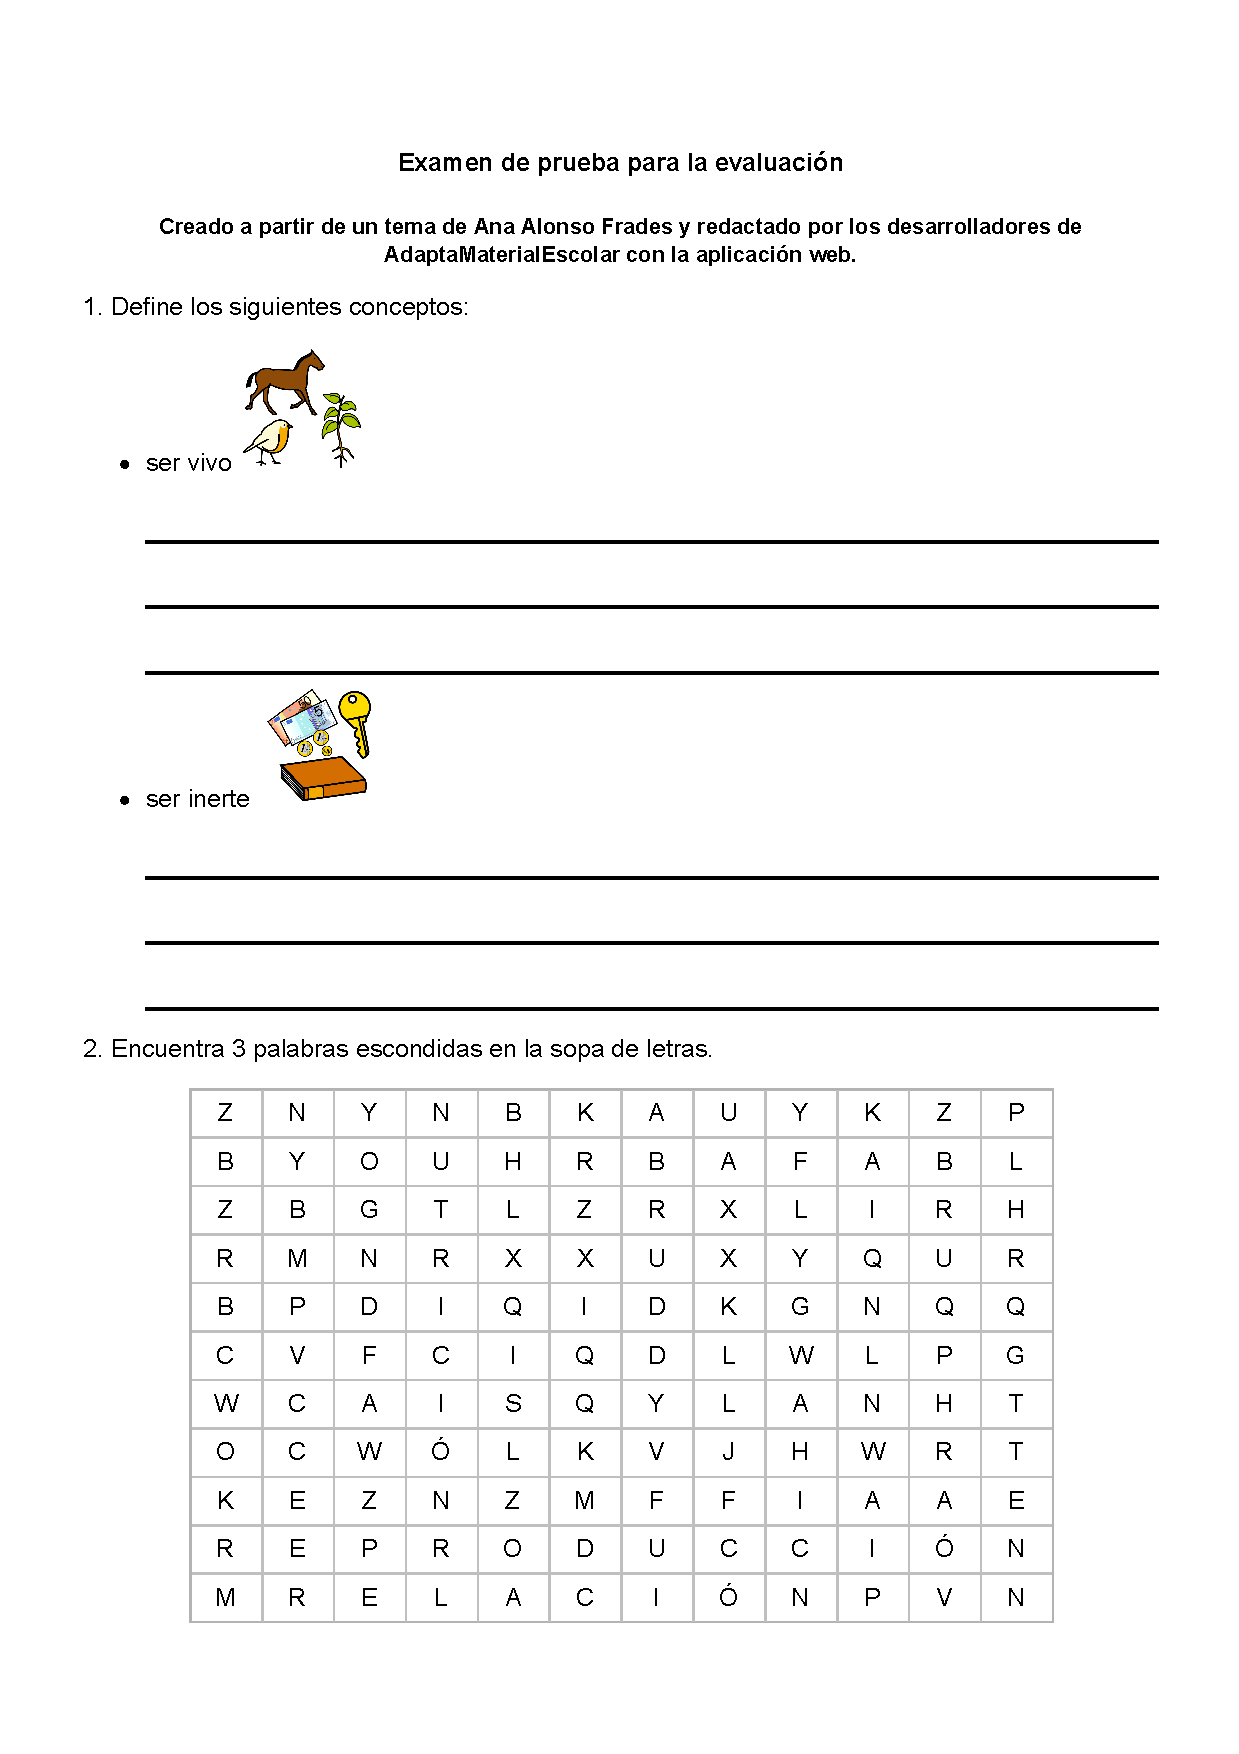
\includegraphics[page=1, width=\textheight]{Apendices/examenprueba.pdf} \\[.5cm]
%		\includegraphics[page=2]{Apendices/examenprueba.pdf}
%	
%	\caption{Examen de prueba para la evaluaci�n}
%	\label{AnexoA:examenprueba}
%\end{figure}

\begin{center}
	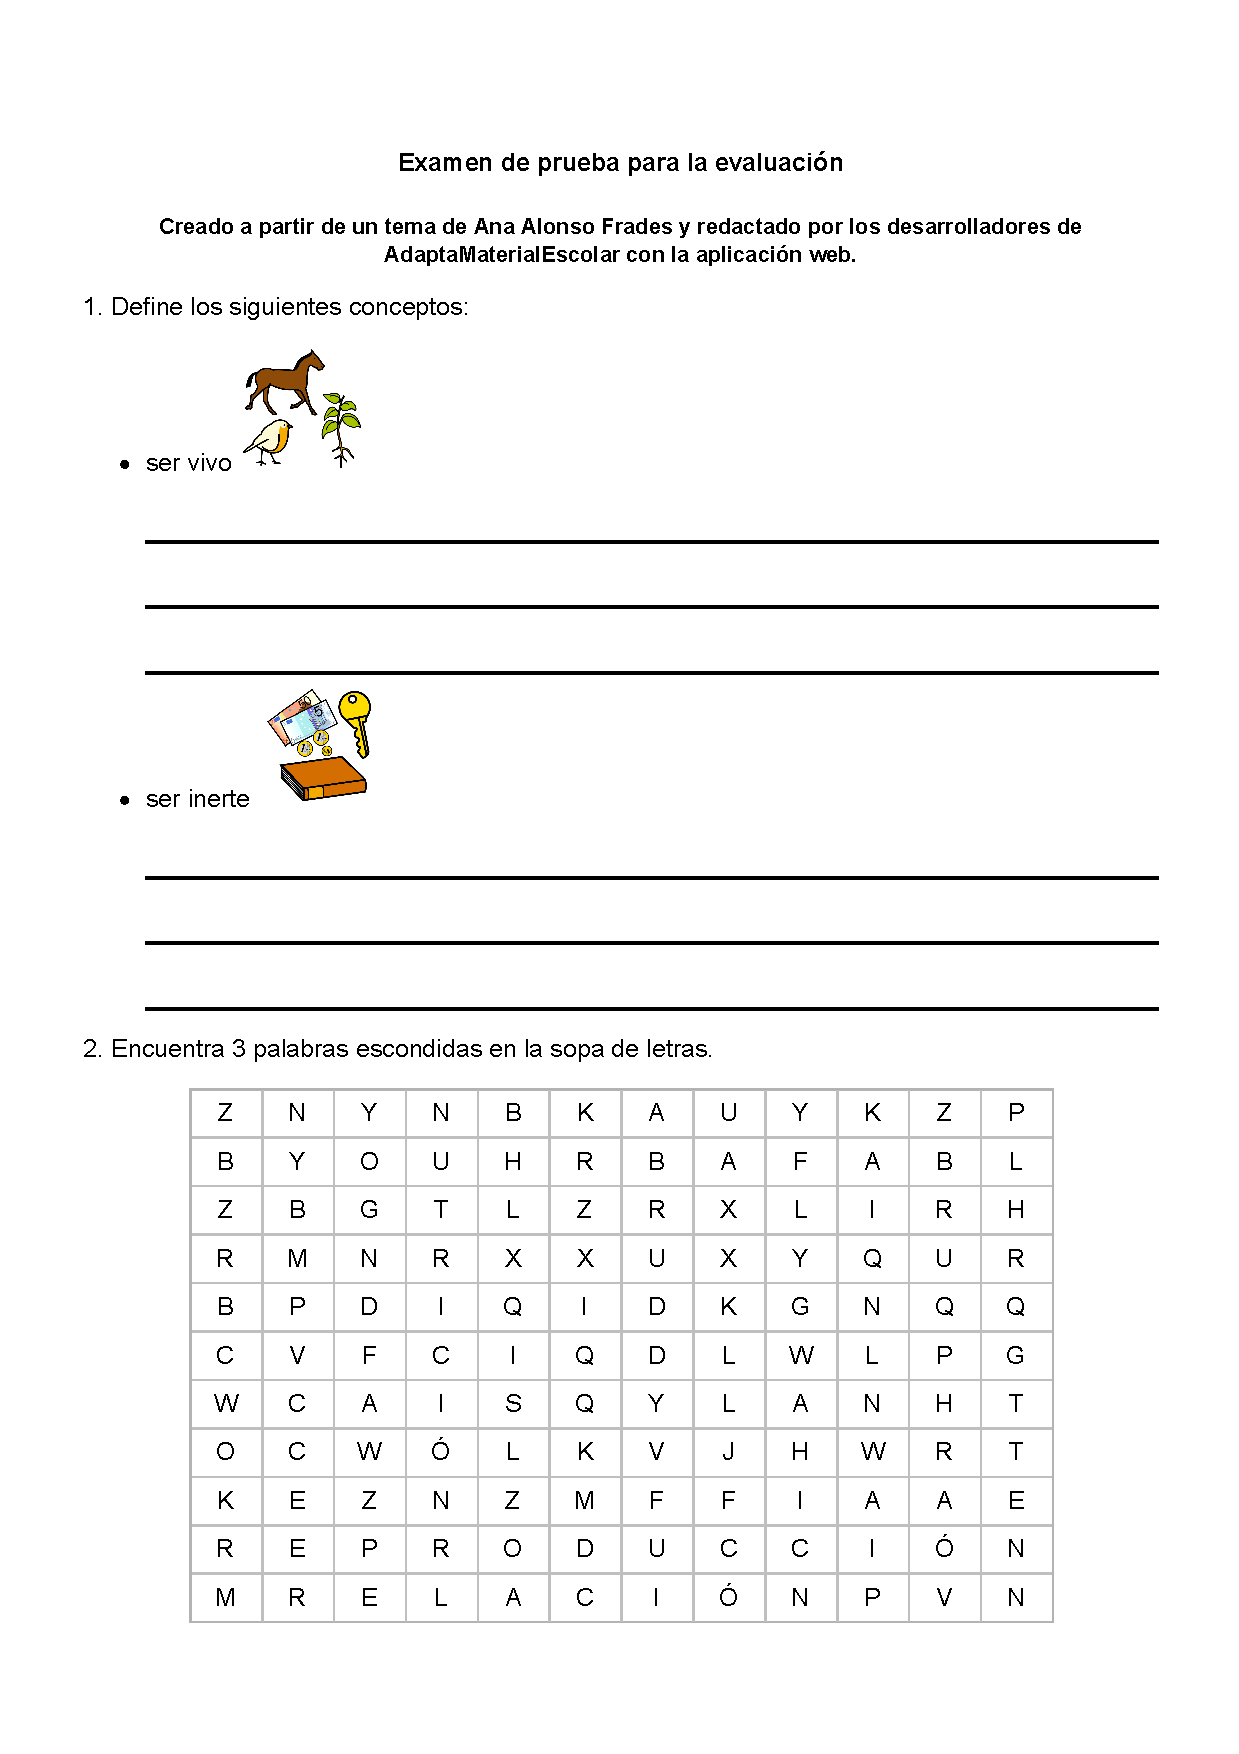
\includepdf[width=\textwidth, height=\textheight, pagecommand={\label{AnexoA:examenprueba}},pages={1,2}]{Apendices/examenprueba}
\end{center}



% Variable local para emacs, para  que encuentre el fichero maestro de
% compilaci�n y funcionen mejor algunas teclas r�pidas de AucTeX
%%%
%%% Local Variables:
%%% mode: latex
%%% TeX-master: "../Tesis.tex"
%%% End:
